\begin{frame}
	\frametitle{Material}
	
	Vídeos para armar estas slides:
	\begin{itemize}
		\item Cyrill Stachniss SLAM \url{https://youtu.be/BuRCJ2fegcc}
		\item Cyrill Stachniss Graph-based SLAM using Pose Graphs \url{https://youtu.be/uHbRKvD8TWg}
		\item Cyrill Stachniss Graph-Based SLAM with Landmarks \url{https://youtu.be/mZBdPgBtrCM}
		\item Cyrill Stachniss Robust Least Squares for Graph-Based SLAM \url{https://youtu.be/z60RbiY18I8}
		\item Cyrill Stachniss Factor Graph \url{https://youtu.be/uuiaqGLFYa4}
		\item Cyrill Stachniss Hierarchical Pose Graphs for SLAM \url{https://youtu.be/uRSow8nMEw8}
		\item Wolfram Burgard, Giorgio Grisetti, and Cyrill Stachniss: Graph-based SLAM \url{https://youtu.be/Alu59K8zvYs}
		\item Frank Dellaert \url{https://youtu.be/tm4E1o11kGo}
        \item Apunte Frank Dellaert and Michael Kaess \url{https://www.cs.cmu.edu/~kaess/pub/Dellaert17fnt.pdf}
	\end{itemize}
	
\end{frame}

\begin{frame}
	\frametitle{Temario para estas slides}
	
	\begin{itemize}
		\item Graph-SLAM / Factor Graph
		\item Loop-Closure
		\item Bundle Adjustment
	\end{itemize}
	
\end{frame}

\begin{frame}
	\frametitle{¿Qué es SLAM?}
	
	Para que un robot móvil pueda navegar de manera autónoma es necesario que conozca su ubicación y cuente con una representación del entorno donde se encuentra. Estos problemas se conocen como el problema Localización y el problema de Mapeo. En el caso más general, donde no se cuenta con un la localización del robot ni con un mapa a priori del entorno, dichas problemas se abordan de manera simultánea. Esto da origen al problema de SLAM (\emph{Simultaneous Localizacion and Mapping}).
	\begin{block}{}
		SLAM es el problema de resolver la localización y el mapeo al mismo tiempo.
	\end{block}
	
\end{frame}


\begin{frame}
    \frametitle{Ejemplo de SLAM}
    
    \begin{figure}
        \subfloat[Realidad]
        {
            \fbox{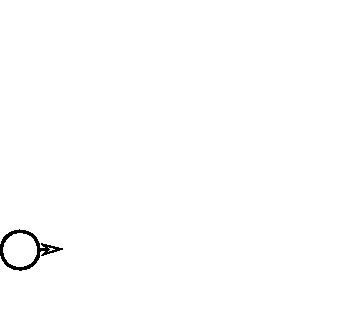
\includegraphics[width=0.44\textwidth]{slam_example_gt1.pdf}}
        }\hfill{}
        \subfloat[Sistema de SLAM del robot]
        {
            \fbox{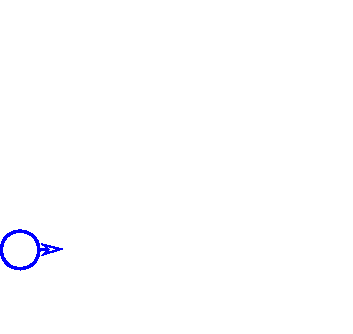
\includegraphics[width=0.44\textwidth]{slam_example_robot1.pdf}}
        }
    \end{figure}
    
\end{frame}

\begin{frame}
    \frametitle{Ejemplo de SLAM}
    
    \begin{figure}
        \subfloat[Realidad]
        {
            \fbox{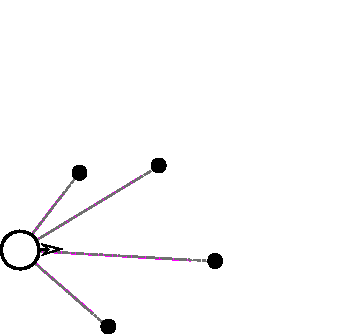
\includegraphics[width=0.44\textwidth]{slam_example_gt2.pdf}}
        }\hfill{}
        \subfloat[Sistema de SLAM del robot]
        {
            \fbox{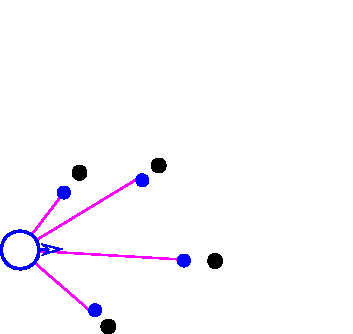
\includegraphics[width=0.44\textwidth]{slam_example_robot2.pdf}}
        }
    \end{figure}
    
\end{frame}

\begin{frame}
    \frametitle{Ejemplo de SLAM}
    
    \begin{figure}
        \subfloat[Realidad]
        {
            \fbox{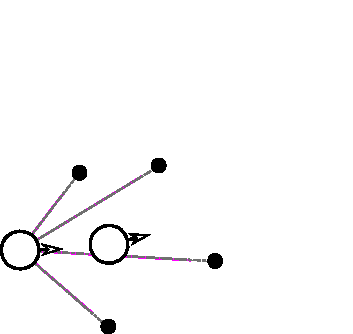
\includegraphics[width=0.44\textwidth]{slam_example_gt3.pdf}}
        }\hfill{}
        \subfloat[Sistema de SLAM del robot]
        {
            \fbox{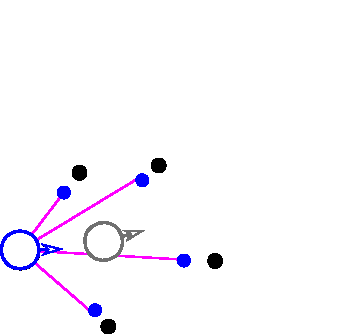
\includegraphics[width=0.44\textwidth]{slam_example_robot3.pdf}}
        }
    \end{figure}
    
\end{frame}

\begin{frame}
    \frametitle{Ejemplo de SLAM}
    
    \begin{figure}
        \subfloat[Realidad]
        {
            \fbox{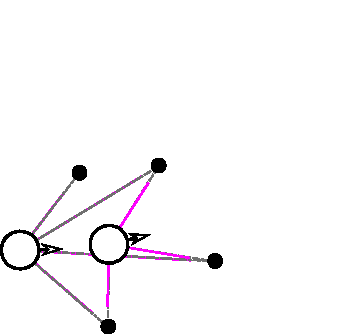
\includegraphics[width=0.44\textwidth]{slam_example_gt4.pdf}}
        }\hfill{}
        \subfloat[Sistema de SLAM del robot]
        {
            \fbox{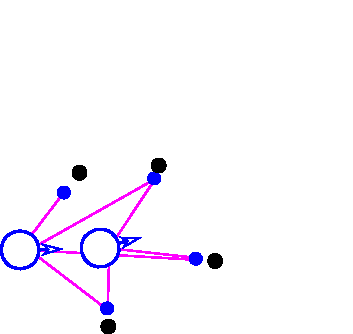
\includegraphics[width=0.44\textwidth]{slam_example_robot4.pdf}}
        }
    \end{figure}
    
\end{frame}

\begin{frame}
    \frametitle{Ejemplo de SLAM}
    
    \begin{figure}
        \subfloat[Realidad]
        {
            \fbox{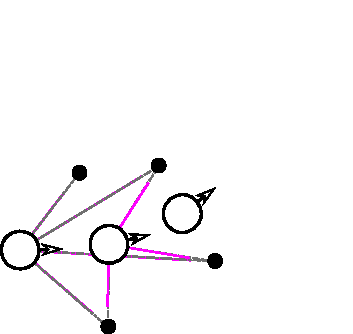
\includegraphics[width=0.44\textwidth]{slam_example_gt5.pdf}}
        }\hfill{}
        \subfloat[Sistema de SLAM del robot]
        {
            \fbox{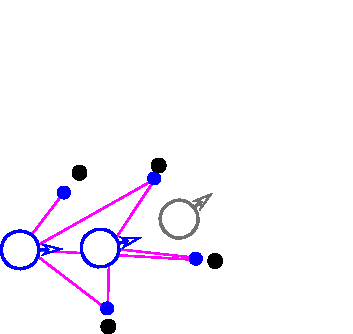
\includegraphics[width=0.44\textwidth]{slam_example_robot5.pdf}}
        }
    \end{figure}
    
\end{frame}

\begin{frame}
    \frametitle{Ejemplo de SLAM}
    
    \begin{figure}
        \subfloat[Realidad]
        {
            \fbox{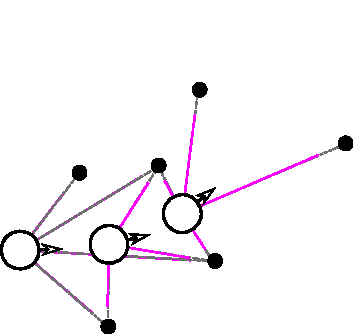
\includegraphics[width=0.44\textwidth]{slam_example_gt6.pdf}}
        }\hfill{}
        \subfloat[Sistema de SLAM del robot]
        {
            \fbox{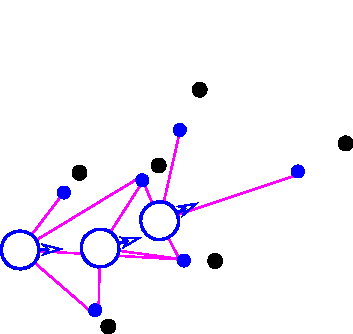
\includegraphics[width=0.44\textwidth]{slam_example_robot6.pdf}}
        }
    \end{figure}
    
\end{frame}

\begin{frame}
    \frametitle{Ejemplo de SLAM}
    
    \begin{figure}
        \subfloat[Realidad]
        {
            \fbox{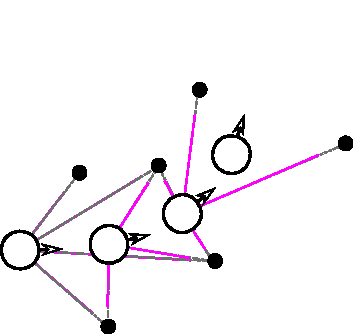
\includegraphics[width=0.44\textwidth]{slam_example_gt7.pdf}}
        }\hfill{}
        \subfloat[Sistema de SLAM del robot]
        {
            \fbox{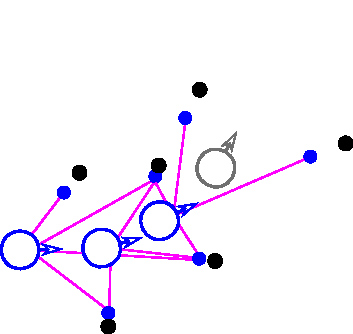
\includegraphics[width=0.44\textwidth]{slam_example_robot7.pdf}}
        }
    \end{figure}
    
\end{frame}

\begin{frame}
    \frametitle{Ejemplo de SLAM}
    
    \begin{figure}
        \subfloat[Realidad]
        {
            \fbox{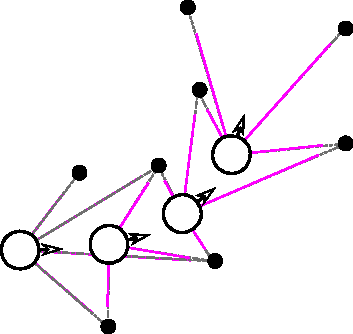
\includegraphics[width=0.44\textwidth]{slam_example_gt8.pdf}}
        }\hfill{}
        \subfloat[Sistema de SLAM del robot]
        {
            \fbox{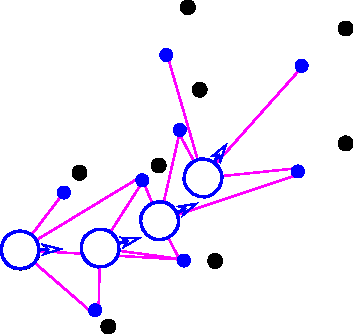
\includegraphics[width=0.44\textwidth]{slam_example_robot8.pdf}}
        }
    \end{figure}
    
\end{frame}

\begin{frame}
	\frametitle{Aquitectura general de SLAM}
	
	\begin{figure}[!h]
			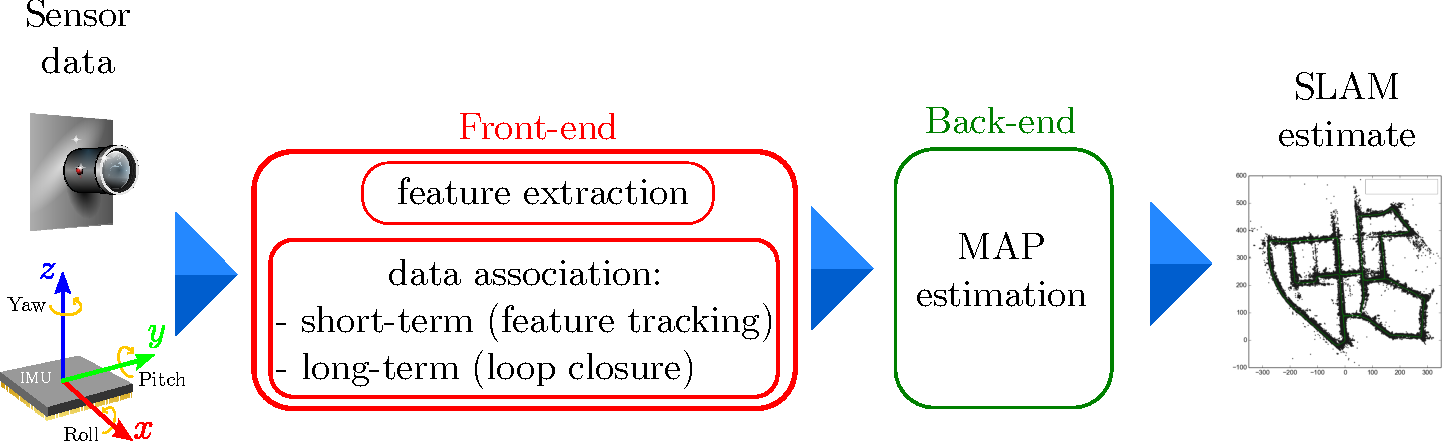
\includegraphics[width=\textwidth]{images/slam_frontend_backend.pdf}
	\end{figure}
	
\end{frame}

\begin{frame}
    \frametitle{Tipos de SLAM Back-ends}
    
    \begin{itemize}
        \item Extended Kalman Filter
        \item Particle Filter (Rao-Blackwellized Particle Filter (FastSLAM))
        \item Least-Squares / Graph-SLAM
        \begin{itemize}
            \item Pose-Graph (solo contiene las poses del robot, el mapa es marginalizado)
            \item Factor-Graph (contiene poses y landmarks)
        \end{itemize}
            Herramientas de optimización
            \begin{itemize}
            \item Ceres
            \item GTSAM
            \item g2o
            \end{itemize}
    \end{itemize}

    \TODO{agregar imagen de grafo de SLAM.}
    
\end{frame}

\begin{frame}
    \frametitle{Graph-SLAM}
    
    Graph-SLAM: construir un grafo y encontrar una configuración de nodos que minimiza el error introducido por las restricciones (aristas)
    
    \begin{itemize}
        \item Se utiliza un grafo para representar el problema.
        \item Los nodos representan poses o ubicaciones de landmarks.
        \item Las aristas son observaciones de landmarks o mediciones de odometría
        \item La minimización optimiza las poses del robot y la ubicación del los landmarks
        \item Observar áreas previamente vistas genera restricciones en el grafo
    \end{itemize}
    
\end{frame}


